
\documentclass{beamer}

\mode<presentation> {

\usetheme{Madrid}

%\usecolortheme{albatross}
%\usecolortheme{beaver}
%\usecolortheme{beetle}
%\usecolortheme{crane}
%\usecolortheme{dolphin}
%\usecolortheme{dove}
%\usecolortheme{fly}
%\usecolortheme{lily}
%\usecolortheme{orchid}
%\usecolortheme{rose}
%\usecolortheme{seagull}
%\usecolortheme{seahorse}
%\usecolortheme{whale}
%\usecolortheme{wolverine}

%\setbeamertemplate{footline} % To remove the footer line in all slides uncomment this line
%\setbeamertemplate{footline}[page number] % To replace the footer line in all slides with a simple slide count uncomment this line

%\setbeamertemplate{navigation symbols}{} % To remove the navigation symbols from the bottom of all slides uncomment this line
}

\usepackage[utf8]{inputenc}
\usepackage[spanish]{babel}
\usepackage[T1]{fontenc}
\usepackage{graphicx}
\usepackage{booktabs} % Allows the use of \toprule, \midrule and \bottomrule in tables
\usepackage{animate} % para crear el gif de kmeans
\usepackage{listings} % para el codigo fuente
\usepackage{hyperref}
%TODO revisar
\hypersetup
{
    %bookmarks=true,         % show bookmarks bar?
    %unicode=false,          % non-Latin characters in Acrobat’s bookmarks
    %pdftoolbar=true,        % show Acrobat’s toolbar?
    %pdfmenubar=true,        % show Acrobat’s menu?
    %pdffitwindow=false,     % window fit to page when opened
    pdfstartview={Fit},    % fits the width of the page to the window
    pdftitle={Estudio comparativo de Algoritmos de machine learning e implementación en Hadoop},    % title
    pdfauthor={David Retana Ribeiro},     % author
    pdfsubject={Big data y machine learning},   % subject of the document
    pdfkeywords={computacion paralela, apache hadoop, apache spark, machine Learning, big data, python, k means,
               naive bayes, yarn, hdfs, cluster}, % list of keywords
    pdfnewwindow=true,      % links in new PDF window
    %colorlinks=true,       % false: boxed links; true: colored links
    %linkcolor=red,          % color of internal links (change box color with linkbordercolor)
    %citecolor=green,        % color of links to bibliography
    %filecolor=magenta,      % color of file links
    %urlcolor=cyan           % color of external links
}

%%%%%%%%%%%%%%%%%%%%%%%%%%%%%%%%%%%%%% TITULO %%%%%%%%%%%%%%%%%%%%%%%%%%%%%%%%%%%%%%%%%%%

\title[Machine Learning y Big Data]{Estudio comparativo de algoritmos de machine learning e implementación en Hadoop}
\author{David Retana Ribeiro}
\institute[UCM]{Universidad Complutense de Madrid \\ \medskip \texttt{davidret@ucm.es}}
\date{3 de Octubre de 2017}

%%%%%%%%%%%%%%%%%%%%%%%%%%%%%%%%%%%%%%%%%%%%%%%%%%%%%%%%%%%%%%%%%%%%%%%%%%%%%%%%%%%%%%%%%

\begin{document}

%%%%%%%%%%%%%%%%%%%%%%%%%%%%%%%%%%%%%%%%%%%%%%%%%%%%%%%%%%%%%%%%%%%%%%%%%%%%%%%%%%%%%%%%%

\begin{frame} % Portada
\titlepage
\end{frame}

%%%%%%%%%%%%%%%%%%%%%%%%%%%%%%%%%%%%%%%%%%%%%%%%%%%%%%%%%%%%%%%%%%%%%%%%%%%%%%%%%%%%%%%%%%

\begin{frame} % Indice de contenidos
\frametitle{Índice de contenidos}
\tableofcontents
\end{frame}

%%%%%%%%%%%%%%%%%%%%%%%%%%%%%%%%%%%%%%%%%%%%%%%%%%%%%%%%%%%%%%%%%%%%%%%%%%%%%%%%%%%%%%%%%%
%%%%%%%%%%%%%%%%%%%%%%%%%%%%%%%%%%%% INTRODUCCION %%%%%%%%%%%%%%%%%%%%%%%%%%%%%%%%%%%%%%%%
%%%%%%%%%%%%%%%%%%%%%%%%%%%%%%%%%%%%%%%%%%%%%%%%%%%%%%%%%%%%%%%%%%%%%%%%%%%%%%%%%%%%%%%%%%

\section{Introducción}

\begin{frame} % Introduccion a Big data y machine learning
  \begin{block}{Big Data}
  Vivimos en la era de los datos, cada día se producen más y más datos  que necesitan ser almacenados y
  procesados para poder sacarles partido.\\
  El termino \textbf{\textit{Big Data}} nace como un concepto para hacer referencia a la incapacidad de 
  los sistemas tradicionales de almacenar y procesar un conjunto masivo de datos.
  \end{block}
  
  \begin{block}{Machine Learning}
  El \textbf{\textit{machine learning}} es una rama de la inteligencia artificial que permite crear sistemas que 
  aprendan automáticamente sin ser programados explícitamente para ello.\\
  Debido a que el \textit{machine learning} se alimenta de los datos, cuantos más datos tengamos para
  entrenar los modelos más preciosos serán estos, por lo que los términos \textit{Big Data} y \textit{machine learning}
  están estrechamente relacionados.
  \end{block}
\end{frame}

%%%%%%%%%%%%%%%%%%%%%%%%%%%%%%%%%%%%%%%%%%%%%%%%%%%%%%%%%%%%%%%%%%%%%%%%%%%%%%%%%%%%%%%%%%

\begin{frame} % Como encajan Hadoop, mapreduce, spark y machine learning al big data
  \frametitle{Herramientas del Big Data}
  Actualmente, existen diversas herramientas que nos permiten trabajar con las grandes cantidades de datos
  manejadas en el \textit{Big Data}. \textit{Apache Hadoop} es el software base que nos permite desplegar
  un cluster de máquinas sobre el que trabajar y desarrollar.\\
  Además de \textit{Hadoop} existen diversas herramientas para numerosos propósitos como pueden ser almacenamiento,
  procesamiento, bases de datos no relacionales (noSQL)...\\
  Entre esas herramientas cabe destacar \textit{Cassandra}, \textit{Apache Spark}, \textit{Hive}, \textit{MongoDB}...
  
\includegraphics[width=0.33\textwidth]{C:/Users/David/Desktop/TFG/TFGLatex/presentacion/recursos/cassandra_logo.png}%
  
\includegraphics[width=0.33\textwidth]{C:/Users/David/Desktop/TFG/TFGLatex/presentacion/recursos/spark_logo.png}%
  
\includegraphics[width=0.33\textwidth]{C:/Users/David/Desktop/TFG/TFGLatex/presentacion/recursos/mongodb_logo.png}
\end{frame}

%%%%%%%%%%%%%%%%%%%%%%%%%%%%%%%%%%%%%%%%%%%%%%%%%%%%%%%%%%%%%%%%%%%%%%%%%%%%%%%%%%%%%%%%%%
%%%%%%%%%%%%%%%%%%%%%%%%%%%%%%%% DESPLIEGUE HADOOP %%%%%%%%%%%%%%%%%%%%%%%%%%%%%%%%%%%%%%%
%%%%%%%%%%%%%%%%%%%%%%%%%%%%%%%%%%%%%%%%%%%%%%%%%%%%%%%%%%%%%%%%%%%%%%%%%%%%%%%%%%%%%%%%%%
\section{Despliegue de un \textit{cluster Hadoop}}

\subsection{\textit{HDFS} y \textit{YARN}}

\begin{frame}[fragile]
\frametitle{HDFS}
\begin{lstlisting}[language=bash, numbers=none, frame=single]
$ hdfs dfs -put <path_archivo_local> <path_hdfs>
\end{lstlisting}
\end{frame}

%%%%%%%%%%%%%%%%%%%%%%%%%%%%%%%%%%%%%%%%%%%%%%%%%%%%%%%%%%%%%%%%%%%%%%%%%%%%%%%%%%%%%%%%%%

\begin{frame}
\frametitle{YARN v2 (\textit{MapReduce} incluido)}
\begin{itemize}
\item Lorem ipsum dolor sit amet, consectetur adipiscing elit
\item Aliquam blandit faucibus nisi, sit amet dapibus enim tempus eu
\item Nulla commodo, erat quis gravida posuere, elit lacus lobortis est, quis porttitor odio mauris at libero
\item Nam cursus est eget velit posuere pellentesque
\item Vestibulum faucibus velit a augue condimentum quis convallis nulla gravida
\end{itemize}
\end{frame}

%%%%%%%%%%%%%%%%%%%%%%%%%%%%%%%%%%%%%%%%%%%%%%%%%%%%%%%%%%%%%%%%%%%%%%%%%%%%%%%%%%%%%%%%%%

\begin{frame} % imagen de topologia de un cluster Hadoop

\end{frame}

%%%%%%%%%%%%%%%%%%%%%%%%%%%%%%%%%%%%%%%%%%%%%%%%%%%%%%%%%%%%%%%%%%%%%%%%%%%%%%%%%%%%%%%%%%
\subsection{\textit{Spark}}

\begin{frame}[fragile]
\frametitle{\textit{Apache Spark}}

\begin{lstlisting}[language=bash, numbers=none, frame=single]
$ pyspark --master yarn-client
\end{lstlisting}

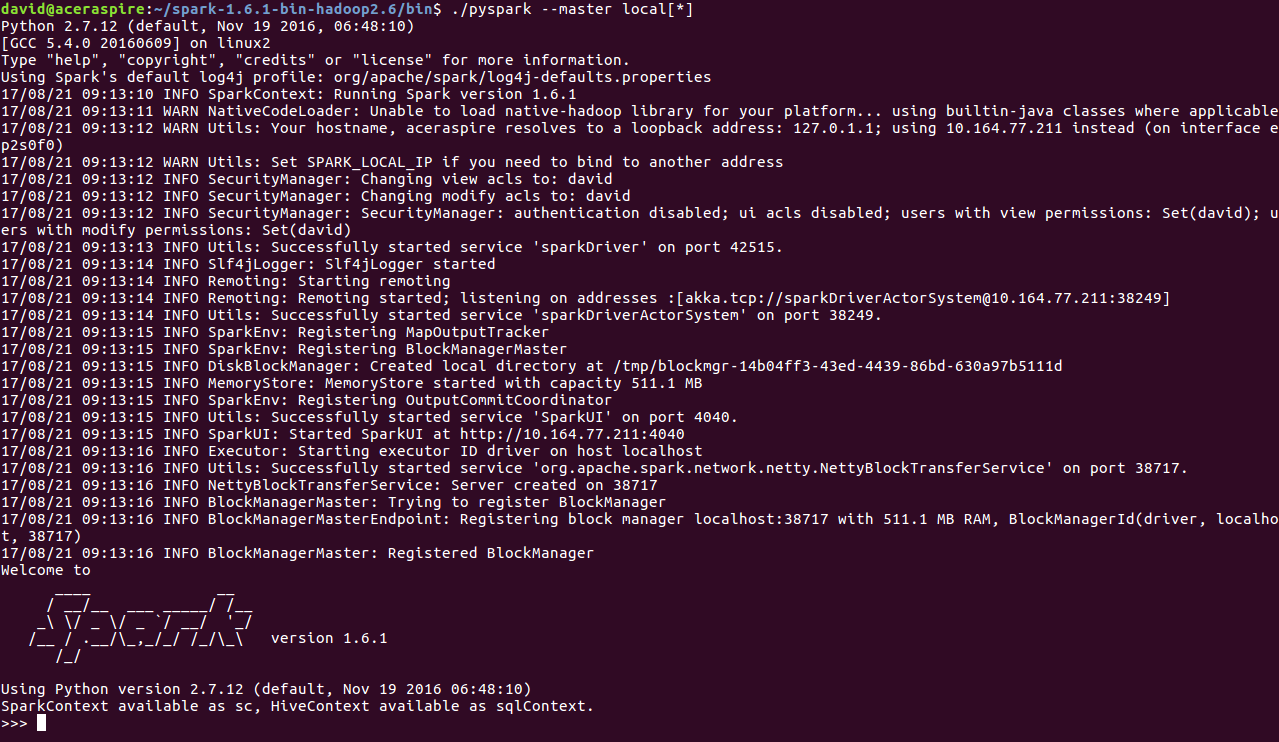
\includegraphics[width=\textwidth]{C:/Users/David/Desktop/TFG/TFGLatex/presentacion/recursos/pyspark_shell.png}

\begin{lstlisting}[language=bash, numbers=none, frame=single, showstringspaces=false]
>>> rdd = sc.parallelize(range(1000))
>>> n = rdd.count()
>>> print("Numero de elementos: ", n)
\end{lstlisting}

\end{frame}

%%%%%%%%%%%%%%%%%%%%%%%%%%%%%%%%%%%%%%%%%%%%%%%%%%%%%%%%%%%%%%%%%%%%%%%%%%%%%%%%%%%%%%%%%%

\begin{frame}
\frametitle{Multiple Columns}
\begin{columns}[c] % The "c" option specifies centered vertical alignment while the "t" option is used for top vertical alignment

\column{.45\textwidth} % Left column and width
\textbf{Heading}
\begin{enumerate}
\item Statement
\item Explanation
\item Example
\end{enumerate}

\column{.5\textwidth} % Right column and width
Lorem ipsum dolor sit amet, consectetur adipiscing elit. Integer lectus nisl, ultricies in feugiat rutrum, porttitor sit amet augue. Aliquam ut tortor mauris. Sed volutpat ante purus, quis accumsan dolor.

\end{columns}
\end{frame}

%%%%%%%%%%%%%%%%%%%%%%%%%%%%%%%%%%%%%%%%%%%%%%%%%%%%%%%%%%%%%%%%%%%%%%%%%%%%%%%%%%%%%%%%%%
%%%%%%%%%%%%%%%%%%%%%%%%%%%%%%%%% MACHINE LEARNING %%%%%%%%%%%%%%%%%%%%%%%%%%%%%%%%%%%%%%%
%%%%%%%%%%%%%%%%%%%%%%%%%%%%%%%%%%%%%%%%%%%%%%%%%%%%%%%%%%%%%%%%%%%%%%%%%%%%%%%%%%%%%%%%%%
\section{Algoritmos de \textit{Machine Learning}}

\begin{frame}
\frametitle{Table}
\begin{table}
\begin{tabular}{l l l}
\toprule
\textbf{Treatments} & \textbf{Response 1} & \textbf{Response 2}\\
\midrule
Treatment 1 & 0.0003262 & 0.562 \\
Treatment 2 & 0.0015681 & 0.910 \\
Treatment 3 & 0.0009271 & 0.296 \\
\bottomrule
\end{tabular}
\caption{Table caption}
\end{table}
\end{frame}

%%%%%%%%%%%%%%%%%%%%%%%%%%%%%%%%%%%%%%%%%%%%%%%%%%%%%%%%%%%%%%%%%%%%%%%%%%%%%%%%%%%%%%%%%%
\subsection{Algoritmo de \textit{NaiveBayes}}

\begin{frame}
\frametitle{Theorem}
\begin{theorem}[Mass--energy equivalence]
$E = mc^2$
\end{theorem}
\end{frame}

%%%%%%%%%%%%%%%%%%%%%%%%%%%%%%%%%%%%%%%%%%%%%%%%%%%%%%%%%%%%%%%%%%%%%%%%%%%%%%%%%%%%%%%%%%

\begin{frame}[fragile] % Need to use the fragile option when verbatim is used in the slide
\frametitle{Verbatim}
\begin{example}[Theorem Slide Code]
\begin{verbatim}
\begin{frame}
\frametitle{Theorem}
\begin{theorem}[Mass--energy equivalence]
$E = mc^2$
\end{theorem}
\end{frame}\end{verbatim}
\end{example}
\end{frame}

%%%%%%%%%%%%%%%%%%%%%%%%%%%%%%%%%%%%%%%%%%%%%%%%%%%%%%%%%%%%%%%%%%%%%%%%%%%%%%%%%%%%%%%%%%

\begin{frame}
\frametitle{Figure}
Uncomment the code on this slide to include your own image from the same directory as the template .TeX file.
%\begin{figure}
%\includegraphics[width=0.8\linewidth]{test}
%\end{figure}
\end{frame}

%%%%%%%%%%%%%%%%%%%%%%%%%%%%%%%%%%%%%%%%%%%%%%%%%%%%%%%%%%%%%%%%%%%%%%%%%%%%%%%%%%%%%%%%%%
\subsection{Algoritmo de \textit{K-Means}}

\begin{frame}[fragile] % Need to use the fragile option when verbatim is used in the slide
\frametitle{Citation}
An example of the \verb|\cite| command to cite within the presentation:\\~

This statement requires citation \cite{p1}.
\end{frame}

\begin{frame} % kmeans gif
  \animategraphics[loop, controls, width=\linewidth]{1} % {n} cuanto menor mas lento
  {C:/Users/David/Desktop/TFG/TFGLatex/presentacion/recursos/kmeans_imagen}{0}{4}
\end{frame}
%%%%%%%%%%%%%%%%%%%%%%%%%%%%%%%%%%%%%%%%%%%%%%%%%%%%%%%%%%%%%%%%%%%%%%%%%%%%%%%%%%%%%%%%%%

\begin{frame}
\frametitle{References}
\footnotesize{
\begin{thebibliography}{99} % Beamer does not support BibTeX so references must be inserted manually as below
\bibitem[Smith, 2012]{p1} John Smith (2012)
\newblock Title of the publication
\newblock \emph{Journal Name} 12(3), 45 -- 678.
\end{thebibliography}
}
\end{frame}

%%%%%%%%%%%%%%%%%%%%%%%%%%%%%%%%%%%%%%%%%%%%%%%%%%%%%%%%%%%%%%%%%%%%%%%%%%%%%%%%%%%%%%%%%%

\begin{frame}
\Huge{\centerline{Fin}}
\end{frame}

%%%%%%%%%%%%%%%%%%%%%%%%%%%%%%%%%%%%%%%%%%%%%%%%%%%%%%%%%%%%%%%%%%%%%%%%%%%%%%%%%%%%%%%%%%

\end{document} 